% This is LLNCS.DEM the demonstration file of
% the LaTeX macro package from Springer-Verlag
% for Lecture Notes in Computer Science,
% version 2.4 for LaTeX2e as of 16. April 2010
%
\documentclass{llncs}
%\usepackage[numbers, sort&compress, square, comma]{natbib}
% \usepackage[lsnumbers, sort&compress, sEquare, comma]{natbib}    
% \usepackage{multirow}                             % not available on your system
\usepackage[table]{xcolor}
% \usepackage{amssymb}
% \usepackage{amsmath}
\usepackage{graphicx}        % standard LaTeX graphics tool                            % when including figure files
\usepackage{multicol}        % used for the two-column index
\usepackage{multirow}
\usepackage{lscape}
\usepackage{float}
\usepackage{url}
\usepackage{caption,subfig}

%            \usepackage[bottom]{footmisc}% places footnotes at page bottom
%            \usepackage{algorithm}
% \usepackage{algorithmic}
% \usepackage{float}
% \usepackage{url}
% \usepackage{caption,subfig}
% \usepackage{textcomp}
% \usepackage{stfloats}
% \usepackage[table]{xcolor}
% \usepackage{lscape}
% \usepackage{type1cm}  
%\usepackage{graphicx}
%\usepackage{makeidx}  % allows for indexgeneration
%
\begin{document}

\mainmatter              % start of the contributions
%
\title{Multi-Objective Divide-and-Evolve: A Hybrid Evolutionary Approach for Solving Temporal Planning Problems}
%
\titlerunning{MODAE for Temporal Planning Problems}  % abbreviated title (for running head)
%                                     also used for the TOC unless
%                                     \toctitle is used
%
\author{Mostepha~R. Khouadjia \inst{1} \and Marc Schoenauer\inst{1}\and
Vincent Vidal\inst{2}  \and Johann Dr\'eo\inst{3} \and Pierre Savéant\inst{3}}
%
\authorrunning{Mostepha~R. Khouadjia et \textit{al.}} % abbreviated author list (for running head)
%
%%%% list of authors for the TOC (use if author list has to be modified)
\tocauthor{Mostepha~R. Khouadjia, Marc Schoenauer, Vincent Vidal, Johann Dr\'eo, and Pierre Sav\'eant}
%
\institute{TAO Project, INRIA Saclay \&  LRI Paris-Sud University, Orsay, France\\%Universit\'{e} Paris-Sud
\email{\{mostepha-redouane.khouadjia, marc.schoenauer\}@inria.fr},\\ %WWW home page:
%\texttt{http://users/\homedir iekeland/web/welcome.html}
\and
ONERA-DCSD, Toulouse, France\\
\email{Vincent.Vidal@onera.fr}\\
 \and
 THALES Research \& Technology, Palaiseau, France\\
 \email{\{johann.dreo, pierre.saveant\}@thalesgroup.com}\\
}

\maketitle              % typeset the title of the contribution

\begin{abstract}

This paper presents and investigates different approaches  based on  Divide-and-Evolve  (DaE) algorithm to solve  multi-objective Temporal Planning Problems (TPPs).
DaE is a hybrid evolutionary algorithm  which splits the initial problem  into several, hopefully easier, sub-problems. The embedded heuristic solver is able  only to solve the ‘small’ problems, and Divide-and-Evolve strategy provides the solution of the whole problem.
This latter is related to transportation problems, where the first objective is the minimization of the travel makespan   and the second one is the minimization of the cost or the risk assigned to the visited cities.
%assigned  to the crossing to visited cities.
%additive or max cost assigned to the visited cities.
% where the first objective is the minimization of the travel makespan   and the second one is the minimization of the cost or  the risk assigned  during the  crossing  of the  visited cities.
We apply  our approaches  on a new set of benchmark test instances and demonstrate their effectiveness to converge toward optimal Pareto front.
 
% \keywords{ Temporal Planning Problems, Divide-and-Evolve, Evolutionary Algorithms,  Multi-objective Optimization. }

\end{abstract}
%
\section{Introduction}

Multi-objective optimization refers to optimizing problems whose formulation involves two or more conflicting objectives, 
which are known as multi-objective optimization
problems (MOPs).
The optimal solution for MOPs is not a single solution, but a set of non-dominated solutions called Pareto optimal solutions.
This set of solutions represents the compromise solutions between the different conflicting objectives. When they are plotted in the objective space they are collectively known as the Pareto front. 
One of the applications in MOPs that has received a growing interest during the last decades is the planning problems.\\
A solution to this class of problems is a sequence of applicable actions mapping an initial state to a goal state.
A subclass of this domain known as Temporal Planning Problems (TPPs) extends the classical planning by adding a duration to actions and by allowing concurrent actions in time.
In the real-world, temporal planning problems require a richer notion of time in which actions can overlap and have different durations. Indeed, other criteria are usually needed to make decision
about the resulting plan as for example its cost or its related risk.\\ 
\indent In the literature, we can find some approaches that have been proposed to solve Multi-Objective Temporal Planning Problems (MOTTP)~\cite{Refanidis2003,Do2003}.
However, these approaches are based on an aggregating methods where the multiple objective functions are combined into a single objective one.
They require multiple runs with different weights for the various objectives in order to find multiple Pareto-optimal solutions.
%allowing single-objective  algorithms to be then applied. These methods require multiple runs with different weights for the various objectives 
%in order to find multiple Pareto-optimal solutions.
During the last decade, the application of metaheuristics to MOPs  and particularly evolutionary algorithms (EAs) have been very successful.
These  approaches use the Pareto dominance concept in their selection process and are an alternative to aggregation-based methods.They offer the advantage of generating multiple Pareto
solutions simultaneously.\\ % As a consequence, many multi-objective EAs have appeared in recent years, and the most well-known metaheuristics, such as NSGA-II~\cite{Deb2002},
%IBEA~\cite{Zitzler2004}, SPEA2~\cite{Zitzler2001} belong to this family. \\
\indent Due to the  high combinatorial complexity and the multi-objective features of TPPs, EAs seem to be good general-purpose candidate 
methods. An approach that has been successfully used on  single-objective temporal planning  problems is \textit{Divide-a-Evolve} (DaE).
Based on the  Divide-and-Conquer paradigm, this generic hybrid evolutionary approach has been originally introduced in~\cite{Schoenauer2006}.   
It splits the problem into a sequence of problems that are hopefully easier to solve by local search based heuristic. 
The initial sequence corresponds to an ordered subgoals to reach which are passed to the embedded heuristic; if all those subgoals are attained, the concatenation of all corresponding sub-plans is a solution of the initial problem.\\
\indent In this paper, we focus on solving MOTTPs by integrating the DAE strategy in  multi-objective evolutionary based metaheuristics.
We compare all these methods to each other on  the transportation Zeno benchmark  test instances and discuss their respective behaviors.
The remainder of the paper is organized as follows: Section~\ref{sec:multi-objective_tpp}  briefly introduces MOTPPS. Section~\ref{sec:evolutionaryMOA}  reviews three  evolutionary metaheuristics for multi-objective optimization. Section~\ref{sec:dae} describes the Divide-and-Evolve strategy, representation, fitness function and variation operators; 
Section~\ref{sec:experimentalpart} is devoted to the experimental part, including the parameter settings and the  analysis of the obtained results.  Finally, Section~\ref{sec:conclusion} presents conclusions and opens some lines for further research.

 


\section{Multi-Objective Temporal Planning Problem}
\label{sec:multi-objective_tpp}

In Artificial Intelligence, planning task can be described by  an initial state, a goal state, and a set of possible actions.  An action can be applied only if certain conditions in the current state are met, and modifies 
the current state when applied. A solution to this class of models is an ordered set of actions mapping the initial state to a goal state.
 
When durations are associated  w the  actions, we face temporal planning in which  actions  can overlap over the time.
In order to  represent a planning problem,  a  formal language  called Planning Domain Definition  Language (PDDL) is used. This latter  has been extended for representing Temporal Planning Problems and is inherited from the STRIPS model.
It was developed mainly to make the International Planning
Competition (IPC) series possible.
Formally,  an action is a tuple $o =\langle pre(o), add(o), del(o), dur(o)\rangle$ where $pre(o)$, $add(o)$ and $del(o)$ are sets of ground atoms that respectively denote the preconditions, adding effects and deleting effects of $a$, and $dur(a)$ is a rational number
that denotes the duration of $a$.   Thus, the planning problem is a tuple $P = \langle A, I, O, G \rangle$ , where $A$ is a set of
atoms representing all the possible facts in a world situation, $I$ and $G$ are two sets of atoms that respectively denote the initial state and the problem goals, and $O$ is a set of actions.
A solution to $P$ is a consistent schedule of  actions whose execution in the initial state leads to a state where the problem goal is satisfied. 
The total duration of the solution plan is called the $makespan$ and its minimization is the usual aim  in single-objective optimization. 
A planning problem defined on domain $D$ with initial state $I$ and goal $G$ will be denoted $P_\textit{D} (I, G)$ in the following.\\
\indent In our context, we deal with Multi-Objective Temporal Planning Problem (MOTPP), the aim to optimize a set of $n \geq 2$ objective functions $f_1 ,f_2, \dots, f_n$ simultaneously.
% Without loss of generality, we assume that all $n$ objective functions have to be minimized. Let $X$ denote the set of feasible solutions in the decision space, and $Z$ the set of feasible points in the objective space. To each decision vector $x \in  X$ is assigned exactly one
% objective vector $z \in Z$ on the basis of a vector function $f : X \rightarrow Z$ with $ z = f (x) = (f1 (x), f2 (x),\dots, fn (x))$. 
A solution $x \in  X $ is said to be  Pareto optimal or  non-dominated  if its mapping in the objective space results in a non-dominated objective vector $z$. 
An objective vector $z \in Z$ is said to dominate  another objective vector $z' \in Z $ iff  $ \forall i \in {1, 2,\dots, n}, z_i \leq z_i'$ and
$\exists j \in {1, 2, \dots, n}$ such as $z_j < z_j'$. \\% An objective vector $z \in Z$ is said to be non-dominated iff there does not exist
%another objective vector $z' \in Z$ such that $z'$ dominates $z$. \\
% The set of all Pareto optimal set is denoted by $X_E$ . The  set of all non-dominated vectors is the \textit{Pareto front}, denoted by $Z_N$.
\indent In this work, we focus on minimizing both the makespan and an additional criterion, that can be interpreted either as a cost, or as a risk: in the former case, this additional objective is an additive measure,
whereas in the latter case (risk) the aggregation function is the max operator. 
For that purpose, we extended  the \textit{Zeno}  transportation domain  which involves transporting people around in planes, the  objectives  are conflicting in the sense that the short path involves higher cost or risk, making the search for a good  trade-off  between both objectives  much harder.\\
\indent Figure~\ref{fig.instance} shows an example:  the only available routes between cities are displayed as edges, only one transportation method is available (plane), and the duration of the transport is shown on the corresponding edge. Risks (or costs) are attached to the cities (i.e., concern any transportation which overflights those cities). In the initial state, the 3 passengers and the 2 planes are in City 0, and the goal is to transport them into City 4.
Going through City 1 is fast, but risky (costly), whereas going through City 3 is slow , but safety.
%We can easily find  three  Pareto-optimal solutions that correspond in the crossing of only one of the middle cities. 
Here, when considering the makespan/cost as objectives, the exact Pareto front is: $(8, 400), (12, 220), (16, 40), (20, 22)$ and $(24, 4)$. 
Whereas for the makespan/risk objectives, we have only three non-dominated vectors that are $(8, 100), (16, 10)$ and $(24, 1)$.
%When all passengers go through respectively City 1, City 2 and City 3, the corresponding values of the makespan and costs in the additive case are (8, 400), (16, 40) and (24, 4), whereas they are, in the max case, (8, 100),
%(16, 10) and (24, 1).
%Furthermore,  it is easy to compute the problem's complexity throughout the  number of possible stations. For instance, with the configuration above: Each passenger can be in one of the 5 cities, or not mentioned (absent predicate). Then,  there are $3^6 = 729$ possible combinations, and $729^n$
%possible lists of length $n$. So, even when $n$ is limited to 6, the size of the search space is is approximating $10^{17}$.\\
 Obtaining the Pareto front of a given MOTTP  is the main goal of multi-objective optimization approaches. 
However, generating the entire set of Pareto optimal solutions is non trivial or infeasible, due to the complexity of
the underlying problem or to the large number of optima. Therefore, the overall goal is often to identify a good efficient set approximation.


\begin{figure}[h]
\begin{center}
 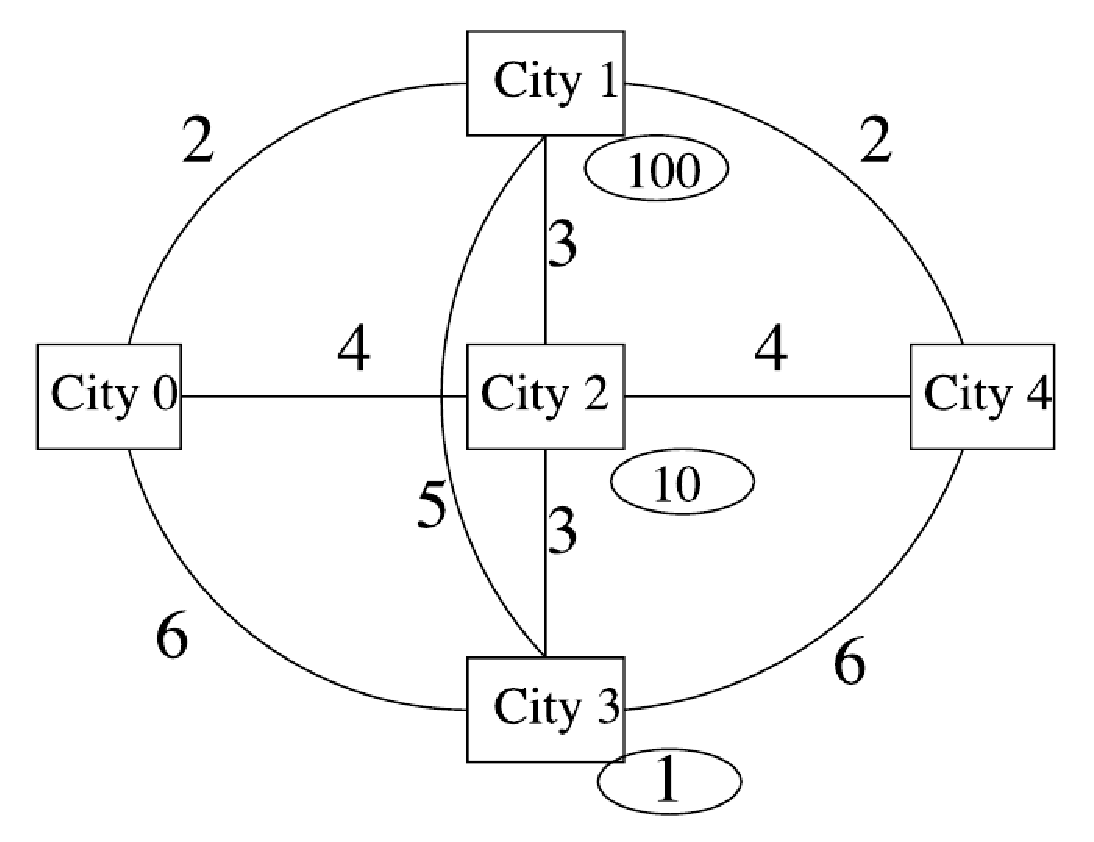
\includegraphics[bb=0 0 509 388,scale=0.35]{./instance.eps}
 % instance.eps: 0x0 pixel, 300dpi, 0.00x0.00 cm, bb=0 0 509 388
\caption{Multi-objective \textit{Zeno} transportation problem: Durations are attached to edges, costs/risks are attached to cities (in circles).}
\label{fig.instance}
\end{center}
\end{figure}



\section{ Evolutionary Multi-Objective Algorithms}
\label{sec:evolutionaryMOA}
%\subsection{NSGA-II:} 
\indent The Non-dominated Sorting Genetic Algorithm (NSGA-II) has been proposed by Deb et \textit{al.}~\cite{Deb2002}. % and it is considered as the most widely used multiobjective resolution method.
At each generation,  the solutions contained in the current  population are ranked into several classes. 
Individuals mapping to vectors from the first front all belong to
the best efficient set; individuals mapping to vectors from the second front all belong to the second best efficient set; and so on.
Two values are then assigned for every solution of the population. The first one corresponds to the rank  the corresponding solution
belongs to, and represents the quality of the solution in terms of convergence. The second one, the crowding distance, consists in
estimating the density of solutions surrounding a particular point of the objective space, and represents the quality of the solution in
terms of diversity.  A solution is said to be better than another solution if it has a best rank value, or in case of equality, if it has
the best crowding distance.\\ %The selection strategy is a deterministic tournament between two random solutions. At the
%replacement step, only the best individuals survive, with respect to the population size. Similarly, an external population is added
%to NSGA-II in order to store every potentially efficient solution found during the search.\\
%\subsection{IBEA:}
\indent Introduced by Zitzler and  K\"uconzli~\cite{Zitzler2004}, the Indicator-Based Evolutionary Algorithm (IBEA)% is a recent method that is a good 
%illustration of the new trend dealing with indicator-based search, and started to become popular in recent years. 
%The principle of IBEA is to 
introduces a total order between solutions by means of a binary quality indicator. 
The fitness assignment scheme of this evolutionary algorithm is based on a pairwise comparison of solutions contained 
in  the current population in regard to a binary quality indicator $I$. For each individual $x$ is assigned a fitness value $F (x)$ measuring the ``loss in quality'' if $x$ was removed from the current
population. Different indicators can be used for such a purpose, and we choose to use mainly the two binary indicators; additive $\epsilon$-indicator ($I_{\epsilon^+}$ ) and the hypervolume
difference indicator ($I_{H^-}$)  as defined in ~\cite{Zitzler2004}. 
Each indicator  $I (x, x')$ gives the minimum value by which a solution $x \in X$  can be translated in the objective space to weakly dominate
another solution $x' \in X$. 
%The selection scheme for reproduction is a binary tournament between randomly chosen individuals. 
%The replacement is based on an iterative elitist strategy that consists in deleting, one-by-one, the worst individuals, and in updating the fitness values of the remaining solutions each time there is a deletion;
%this is iterated until the required population size is reached.  Moreover, 
An archive stores solutions mapping to potentially non-dominated points in order to prevent their loss during the stochastic search process. \\
%\subsection{SPEA2:} 
\indent SPEA2 is considered as an extension of the Strength Pareto Evolutionary Algorithm (SPEA)~\cite{Zitzler2002}, where an improved fitness assignment strategy is proposed. It intrinsically handles an internal archive of fixed size that is used during
the selection step to create offspring solutions. At a given iteration of the algorithm, to each population and archive member $x$ is assigned a strength value $S(x)$ representing the number
of solutions it dominates. Then, the fitness value $F (x)$ of solution $x$ is calculated by summing the strength values of all individuals solution $x$ currently dominates. Additionally,
a diversity preservation strategy, based on a nearest neighbor technique, is incorporated.
The selection step consists of a binary tournament with replacement applied on the internal archive only.
At last, given that the SPEA2 archive has a fixed size storage capacity, a bounding mechanism based on fitness and diversity information is used when the size of
the non-dominated set is too high. %On the contrary, when the size of the non-dominated set is too small. Some dominated solutions are allowed to be incorporated.

\section{Divide-and-Evolve Paradigm}
\label{sec:dae}
The basic idea of DaE in order to solve a planning task ${\cal P}_D(I,G)$ is to find a sequence of states $S_1, \ldots, S_n$, and to use some embedded planner to solve the series of planning problems ${\cal P}_D(S_{k},S_{k+1})$, for $k \in [0,n]$ 
(with the convention that $S_0 = I$ and $S_{n+1} = G$).
The generation and optimization of the sequence of states $(S_i)_{i \in [1,n]}$  is driven by an evolutionary algorithm, where the   sequence of subproblems ${\cal P}_D(S_{k},S_{k+1})$ are solved by an external 'embedded'
planner. The concatenation of the corresponding plans  (possibly with some compression step) is a solution of the initial problem.\\
\indent In this section, we  describe the main components of DaE paradigm that have been integrated in our work into the conventional multi-objective approaches: NSGA-II, IBEA and SPEA2.   
These  components cover: problem-specific representation, variation operators and  the hybridization with the embedded planner.

\subsection{Representation}
\indent An individual is considered as a  possible solution of the MOTPP at hand and is a  list (variable length) of subgoals, or partial states of the given domain.
In STRIPS representation model~\cite{Fikes1971}, a state is a list of boolean atoms.  
%However, searching the space of complete states would result in a rapid explosion of the size of the search space. Moreover, goals of
%planning problem need only to be defined as partial states. It thus seems more practical to search only sequences of partial states,
%and to limit the choice of possible atoms used within such partial states. However, this raises the issue of the choice of the atoms to be used to represent individuals, among
%all possible atoms. 
The result of the previous experiments on different domains of temporal planning tasks from the
IPC benchmark series demonstrates the need for a very careful choice of the atoms that are used to build the partial states. 
The method used to build the partial states are based on an estimation of the earliest time from which an atom can become true. %Such estimation can be obtained
%by any admissible heuristic function (e.g $h^1$, $h^2$, $\ldots$~\cite{Haslum2000}). 
The possible start times are then used in order to restrict the candidate atoms for each partial state. A partial state is built at a given time by randomly choosing among several atoms that are possibly true at this time. The sequence of
states is then built by preserving the estimated chronology between atoms (time consistency). %Heuristic function $h^1$ has been used for all experiments presented here. 
An individual in DaE is hence represented as a variable length ordered time-consistent list of partial states, and each state is a variable-length list of atoms that are not pairwise mutex. Furthermore, all operators that manipulate the representation (see below) maintain the chronology between atoms and the local consistency of a state, i.e. avoid 
pairwise mutexes.

\subsection{Initialization \& Variation Operators }
The initialization of an individual is the following: first, the number of states is uniformly drawn between 1 and the number of estimated start times; For every chosen time, the number of atoms per state is uniformly chosen between 1 and the number of atoms of the corresponding restriction.
Atoms are then chosen one by one, uniformly in the allowed set of atoms, and added to the individual if not mutex with any other atom that is already there.
One-point crossover is used, adapted to variable-length representation in that both crossover points are independently chosen, uniformly in both parents.
Four different mutation operators have been designed, and once an individual has been chosen for mutation (according to a population-level mutation rate),
the choice of which mutation to apply is made according to user-defined relative weights.
%Because an individual is a variable length list of states, and a state is a variable length list of atoms,
The mutation operator can act at both levels: at the individual level by adding (addState) or removing (delState) a state; or at the state level by adding (addAtom) or removing (delAtom) some atoms in the given
state. Note that the initialization process and these variation operators maintain the chronology between atoms in a sequence of states and the local consistency 
of a state, i.e. avoiding pairwise mutexes.
\subsection{Hybridization}

Our algorithms have been hybridized with an external ’embedded’ planner to solve the sequence of problems ${\cal P}_D(S_{k},S_{k+1})$,  for $k \in [0,n]$. 
Any existing planner can be used as embedded planner, but since guaranty of optimality at all calls is not mandatory in order for DaE to obtain good quality results~\cite{Bibai2010}, a sub-optimal, but fast planner is used: YAHSP~\cite{Vidal2004} is a lookahead 
strategy planning system for sub-optimal planning which uses the  actions in the relaxed plan to compute reachable states in order to speed up the search process.\\ 
For any given $k$, if the chosen embedded planner succeeds in solving $ P_{D} (S_k, S_{k+1} )$, the final complete state is computed by executing the solution plan
from $S_k$ , and becomes the initial state of the next problem. If all the subproblems are solved by the  embedded planner, 
the individual is called \textit{ feasible}, and the concatenation of  the found  subplans for all subproblems  is a
global solution plan for $P_{D} (S_{0} = I, S_{n+1} = G)$. However, this plan can in general be further optimized by rescheduling some of its actions, in a step called
compression. The computation of both objective values (makespan and risk/cost) is done from the compressed plan of the given individual.
% However, as soon as the chosen embedded planner fails to solve one $ P_{D} (S_k, S_{k+1} )$  subproblem, the following subproblem $ P_{D} (S_k+1, S_{k+2} )$ cannot be even tackled
% by the chosen embedded planner, as its initial state is in fact partially unknown.
% Hence no quality in term of number of action, cost or makespan can be given to this individual. All such individuals receive a fitness that is higher than that
% of any feasible individual. Furthermore, in order to nevertheless give some selection pressure toward feasible individuals, such fitness takes into account the
% proportion of subproblems solved. 
% Finally, because the initial population contains randomly generated individuals, some of them might contain some subproblems that are in fact more difficult
% than the original global problems. It was thus necessary to limit the embedded planner by imposing some complexity bound in order to discard too difficult
% subproblems.
%  However, though it is hoped that all subproblems will ultimately be easy to solve, such limitation should not be too strong in order to nevertheless
% leave some degree of freedom to the search for solutions. Here,  YAHSP  has been limited by a maximal number of backtracks (resp. a maximal number of nodes) that it is allowed to use to
% solve any of the subproblems. Those bounds are determined  for each run by a two-step process: first, the initial population is evaluated using a very high
% bound (e.g. 10e4 backtracks or nodes); the bounds for the rest of the run are then chosen as the median of the actual number of backtracks (resp. nodes) that
% have been used to find the solutions during these initial evaluations.
Finally, the embedded planner has been limited by a maximal number of backtracks (resp. a maximal number of nodes) that it is allowed to use to solve any of the subproblems.

\section{Experimental Analysis}
\label{sec:experimentalpart}
In this section, we present an experimental analysis of the proposed approaches applied on MOTTP benchmark set. Furthermore, we assess the performance of our algorithms according to quality indicator.
The proposed approaches has been implemented within the ParadisEO-MOEO framework~\footnote{http://paradiseo.gforge.inria.fr/}.% This latter is a $C++$  white-box object-oriented framework dedicated to the reusable design of metaheuristics
%for multi-objective optimization.

\subsection{Benchmark Set \&  Parameter Tunning}
Experiments have been conducted  on the  multi-objective Zeno benchmark set. Initially proposed in~\cite{Schoenauer2006}, we extend the existing set by increasing the number of passengers to carry.
These  instances contain between 3 and 9 passengers and 3 cities. 
Furthermore, for each instance we deal both with the additive case (cost)  and the maximum case (risk) for the second objective to minimize in addition to the makespan as first objective.
So at the end , we have 3 instances with two variants for each one.
The name of each instance indicates the number of the passengers and the case  to deal as second objective.
%The parameter settings used in the experiments are summarized in Table~\ref{table:parameters}. 
The default parameter values are taken from the reference paper where the DaE algorithm is described~\cite{Bibai2010}.%{Bibai2009}.
Besides, the population size has been set to $100$ individuals, where the stopping condition is $1000$ generations.
Furthermore,  the embedded planner YAHSP  is constrained with a maximal number of expanded nodes. Depending on the complexity of the planning task, this number varies
from few  to thousands nodes.% In our work this parameter takes values in the range $[10e4, 10e6]$.
%However, since our instances are relatively small, we have fixed this number to  $10^6$ .
% \begin{table*}[h]
% \centering
% \scriptsize
% \begin{tabular}{l c c c}
% \hline\hline
% Name & Min & Max & Default \\ 
% \hline
% Probability of crossover & 0.0 & 1 & 0.8 \\
% Probability of mutation & 0.0& 1& 0.2 \\
% Rate of mutation add station& 0& 10& 1 \\
% Rate of mutation delete station& 0& 10& 3 \\
% Rate of mutation add atom& 0& 10& 1 \\
% Rate of mutation delete atom& 0& 10& 1 \\
% Mean average for mutations& 0.0& 1& 0.8 \\
% %Time interval radius& 0& 10& 2 \\
% %Maximum number of stations& 5& 50& 20 \\
% Maximum number of nodes & 100& 10e6& 10e4 \\
% %Population size& 10& 300& 100 \\
% %Number of offspring & 100& 2 000& 700 \\
% \hline
% \end{tabular}
% \caption{Algorithm parameters}
% \label{table:parameters}
% \end{table*} 
\subsection{Results and Discussion}
Results obtained on zeno instances  differ from each an other according to  the  size of the instances as well as the  considered second objective.
Indeed, as shown in the figure~\ref{fig:zenoParetofront}, when  considering  the cost as second objective, 
SPEA2 has  both better convergence and distribution than the other algorithms.
On  the instance  Zeno3, SPEA2 and IBEA$_{\epsilon^+}$ success in finding the  exact Pareto front  which consists in five solutions (see Section~\ref{sec:multi-objective_tpp}), while NSGAII and IBEA$_{H^-}$  have found only four non-dominated solutions.
Concerning  zeno6 and  zeno9,  SPEA2 and IBEA$_{H^-}$  algorithms have better Pareto front compared to NSGA and IBEA$_{\epsilon^+}$.
Moreover, when considering the risk as the second objective, we noticed the same observation as for zeno3, while for zeno6  and zeno9, the algorithms find only one solution among the three of the true Pareto front.% 


% For all \textit{Zeno} instances, we can observe that the fronts obtained by SPEA2 has a better convergence and distribution of solutions than the other ones. 
% Besides, in the case of $Zeno3$, all the solutions have converged towards the true Pareto front, while in NSGA-II and IBEA$_{H^-}$ fronts some 
% solutions have not. For the instance $Zeno6$, the fronts are quite similar between them, although we can appreciate some slight differences.\\

% For both instances, we can observe that the fronts obtained by IBEA$_{\epsilon^+}$ and SPEA2 have a better convergence and distribution of solutions than the other ones. 
% Besides, in the case of $Zeno3$, all the solutions have converged towards the true Pareto front, while in NSGA-II and IBEA$_{H^-}$ fronts some 
% solutions have not. For the instance $Zeno6$, the fronts are quite similar between them, although we can appreciate some slight differences.\\
The evolution of the quality of solutions is computed according to $I_{H^-}$ indicator and is depicted for each instance in Figure~\ref{fig:zenoHypervolume}.
In detail, the curves of Figure~\ref{fig:zenoHypervolume}(a,b) and Figure~\ref{fig:zenoHypervolume}(c,d) are 
respectively obtained on the instance $Zeno3$ and $Zeno6$ by considering the second objective as total cost or risk.
At first sight, the outcomes obtained show that algorithms converge far more quickly towards the optimal Pareto front  when considering the
total cost case than in the risk case.
In detail, we can see that a great part of the optimization is achieved around the first 400  and 50 generations respectively for the cost and risk case and that the improvement of the quality of solutions is quite slow after these generations.
Depending on the instance, we can see that two different scenarios:
When dealing with the total cost case (Figure~\ref{fig:zenoHypervolume}(a,c)), it seems that for the instance $zeno3$ SPEA2 and IBEA$_{\epsilon^+}$ outperform NSGA-II and IBEA$_{H^-}$.
While, on the instance $zeno6$, it appears that the previous observation is reversed. Indeed, the results of NSGA-II and IBEA$_{H^-}$ are quite equivalent
and outperform those of SPEA2 and IBEA$_{\epsilon^+}$.\\
%If we are now interested in the realistic instances (Fig. 10(c, d)), the quality of solutions follows practically the
However, when considering the risk case (Figure~\ref{fig:zenoHypervolume}(b,d)), the quality of solutions  for all algorithms 
follows practically the same evolution. Even if the  convergence of SPEA appears to be a bit slower than the other algorithms.
It is interesting to note that the size of instances  and the  second  considered objective, seem  influence the efficiency of the algorithms.
SPEA2 and IBEA$_{\epsilon^+}$  provide  better solutions on small instances,  where, NSGA-II and IBEA$_{H^-}$ have better convergence and distribution  towards the optimal Pareto front on 
larger instances. However, the performances are similar when considering the risk as a second objective.
%Depending on the instance, we can see that two different scenarios:
\subsection{Performance Assessment}
 A set of 30 runs per instance has been performed for each algorithms. % In order to evaluate the quality of the approximations for every
%instance, we follow the protocol proposed in~\cite{Fonseca2005}.
% For a given instance, let $Z^{all}$ denote the union of the outputs that
% we obtained during all our experiments. Note that this set probably contains both dominated and non-dominated points, as a given approximation may contain
% vectors dominating the ones of another approximation, and vice versa.\\
% We first compute a reference set $Z^*_N$ containing all the non-dominated points of $Z^{all}$. 
% Second, we define $z^{min} = (z^{min}_1 ,\ldots, z^{min}_n)$ an $z^max =(z^{max}_1 ,\ldots, z^{max}_n)$, where $z^{min}_k$ (resp. $z^{max}_k$) denotes the lower (resp. upper)
%  bound for the $k^{th}$ objective for all the points contained in $Z^{all}$.
% In order to give a roughly equal range to the objective functions, values are normalized with respect to $z^min$ and $z^{max}$.
% Then, to measure the quality of an output set $A$ in comparison to $Z^*_N$ , we compute the difference between these two sets by using the unary hypervolume
% metric~\cite{Zitzler2004}, $z^{max}$ being the reference point. 
In order to measure the quality of an output set of solutions $A$ in comparison to a reference set $Z^*_N$, we compute the difference between these two sets by using the unary hypervolume
metric~\cite{Zitzler2004}. The hypervolume computes the volume (in objective function space) comparatively to $Z^*_N$. The closer this measure to 0, the better is the approximation $A$.
%. The hypervolume difference indicator ($I^-_H $) computes the portion of the objective
%space that is weakly dominated by $Z^*_N$ and not by $A$. The closer this measure to 0, the better is the approximation $A$~\cite{Zitzler2004}.
% Furthermore, we also consider the additive $\epsilon$-indicator proposed in~\cite{Zitzler2004}. %The unary additive $\epsilon$-indicator ($I^1_{\epsilon^+}$ ) gives the minimum factor by which an approximation $A$ has to be translated in the objective
%space to dominate the reference set $Z^*_N$. 
%Note that both $I^-_H $  and $I^1_{\epsilon^+}$ values are to be minimized. and $I^1_{\epsilon^+}$  measures
Thus, for each test instance, we obtain 30 $I^-_H $ measures  corresponding to the 30  runs performed for each algorithm. 
Once all these values are computed, we perform a statistical analysis for a pairwise comparison of methods. To this end, we use the Wilcoxon signed rank test. For a given
test instance, and with respect to a confidence level of $95~\%$ (\textit{p}-value of 0.05) and according to the metric under consideration, this statistical test reveals if
the sample of approximation sets obtained by a given search method is significantly better than the one of another search
method, or if there is no significant difference between both of them. Note that all the performance assessment procedures have been achieved using
the performance assessment tool suite provided in PISA~\footnote{http://www.tik.ee.ethz.ch/pisa/}.%~\cite{Bleuler2003}.
\begin{table*}[h]
\scriptsize
\caption{Algorithms comparison according to Wilcoxon signed rank test with respect of the I$_{H^-}$ metric.}
\label{table:tests}
\centering

\begin{center}
\scriptsize
\begin{tabular}{|l|l|c|c|c|c|c|}

   \hline
    \multirow{2}*{Instances}  &  \multirow{2}*{Algorithms}	&  \multirow{2}*{Average}	&  \multicolumn{4}{c|}{ Algorithms}\\
    \cline{4-7}
			      &            		 	& 		      		& $NSGAII$  &  $IBEA_{\varepsilon}$ &$IBEA_{\textit{H}}$  & $SPEA2$  \\
   \hline
  \multirow{4}*{\textit{Zeno3}$_{cost}$} &$NSGAII$       	&  6.21e-02  &  --     & 		$\equiv$     &  	$\equiv$   	&  	$\equiv$   \\
				
			      &  $IBEA_{\varepsilon^+}$  	&  5.26e-02 			& $\equiv$  	   & 	--       		& 	$\equiv$ 	&	$\equiv$      \\
			      &    $IBEA_{H^-}$   	 	&    5.92e-02    	& 	$\equiv$  	&		$\equiv$  &--	&	$\equiv$    \\
			      &    $SPEA2$       		& 5.30e-02 			& $\equiv$ 		&	$\equiv$ 	&	$\equiv$  			 &  --  \\
  \hline
  \multirow{4}*{\textit{Zeno3}$_{risk}$} & $NSGAII$ 	&  3.28e-01   			&		-- 					&$\equiv$  		& $\equiv$  	& $\equiv$ \\
	      & $IBEA_{\varepsilon^+}$   	   	 	&     3.70e-01		&$\equiv$ 						&-- 			&$\equiv$  	&  $\equiv$  \\
	      &  $IBEA_{H^-}$ &     4.06e-01   		&$\equiv$ 			& $\equiv$  						&-- 	 & $\equiv$   \\
	      &  $SPEA2$  &     3.52e-01   		&$\equiv$  & $\equiv$ 			&$\equiv$  & --   \\
 \hline
\hline
  \multirow{4}*{\textit{Zeno6}$_{cost}$} &$NSGAII$       	& 1.93e-01	&  --  			   & 		$\equiv$       &  $\equiv$  	&  $\equiv$  	   \\
				
			      &  $IBEA_{\varepsilon^+}$  	&  2.07e-01			& $\equiv$      	   & 	--       		& 	$\equiv$ 	&	$\equiv$      \\
			      &    $IBEA_{H^-}$   	 	&  1.99e-01   		& $\equiv$  		& 	$\equiv$ 	&	--		& $\equiv$   \\
			      &    $SPEA2$       		& 1.96e-01    			&  $\equiv$  		&	$\equiv$ 	&	$\equiv$ 		 &  --  \\
  \hline
 \multirow{4}*{\textit{Zeno6}$_{risk}$} &$NSGAII$       	&  5.55e-01  			&  --  			   & 		$\equiv$       &  	$\equiv$ &  	 	\cellcolor [gray]{0.8}$\succ$      \\
				
			      &  $IBEA_{\varepsilon^+}$  	&   5.55e-01
		& $\equiv$      	   & 	--       		& 	$\equiv$ 	&	\cellcolor [gray]{0.8}$\succ$     \\
			      &    $IBEA_{H^-}$   	 	&   5.55e-01     		& $\equiv$ 		& 	$\equiv$ 	&	--		& \cellcolor [gray]{0.8}$\succ$  \\ %(0.001) 
			      &    $SPEA2$       		& 5.59e-01
   			& 	$\prec$		&		$\prec$		&		$\prec$			 &  --  \\
 
  \hline
\hline
  \multirow{4}*{\textit{Zeno9}$_{cost}$} &$NSGAII$       	& 2.27e-01	&  --  			   & 		$\equiv$       &  $\equiv$  	&  $\equiv$  	   \\
				
			      &  $IBEA_{\varepsilon^+}$  	&  2.23e-01
			& $\equiv$      	   & 	--       		& 	$\equiv$ 	&	$\equiv$      \\
			      &    $IBEA_{H^-}$   	 	& 2.23e-01  		& $\equiv$  		& 	$\equiv$ 	&	--		& $\equiv$   \\
			      &    $SPEA2$       		& 2.47e-01
    			&  $\equiv$  		&	$\equiv$ 	&	$\equiv$ 		 &  --  \\
  \hline
 \multirow{4}*{\textit{Zeno9}$_{risk}$} &$NSGAII$       	&  5.56e-01 			&  --  			   & 		$\equiv$       &  	$\equiv$ &  	 	\cellcolor [gray]{0.8}$\succ$      \\
				
			      &  $IBEA_{\varepsilon^+}$  	& 5.56e-01
		& $\equiv$      	   & 	--       		& 	$\equiv$ 	&	\cellcolor [gray]{0.8}$\succ$      \\
			      &    $IBEA_{H^-}$   	 	& 5.56e-01     		& $\equiv$ 		& 	$\equiv$ 	&	--		& \cellcolor [gray]{0.8}$\succ$    \\
			      &    $SPEA2$       		& 5.59e-01

   			& 	$\prec$		&		$\prec$		&		$\prec$			 &  --  \\
 
  \hline
\end{tabular} 

\end{center}
\end{table*}
%
%% \begin{landscape}
%\begin{table*}[ht!]
%\caption{Algorithms comparison according to Wilcoxon signed rank test with respect of the I$_{\varepsilon^+}^{1}$ metric.}
%\label{table:tests}
%\centering
%\scriptsize
%\begin{center}
%
%\begin{tabular}{|l|l|c|c|c|c|c|}
%   \hline
%    \multirow{2}*{Instances}  &  \multirow{2}*{Algorithms}	&  \multirow{2}*{Average}	&  \multicolumn{4}{c|}{ Algorithms}\\
%    \cline{4-7}
%			      &            		 	& 		      		& $NSGAII$  &  $IBEA_{\varepsilon}$ &$IBEA_{\textit{H}}$  & $SPEA2$  \\
%   \hline
%  \multirow{4}*{\textit{Zeno3}$_{cost}$} &$NSGAII$       	&  6.21e-02  &  --     & 		$\equiv$     &  	\cellcolor [gray]{0.8}$\succ$ (0.05) 	&  	$\equiv$   \\
%				
%			      &  $IBEA_{\varepsilon^+}$  	&  5.26e-02 			& $\equiv$  	   & 	--       		& 	$\equiv$ 	&	$\equiv$      \\
%			      &    $IBEA_{H^-}$   	 	&    5.92e-02    	& 	$\prec$		&		$\equiv$  &--	&	$\prec$	  \\
%			      &    $SPEA2$       		& 5.30e-02 			& $\equiv$ 		&	$\equiv$ 	&	\cellcolor [gray]{0.8}$\succ$(0.025)			 &  --  \\
%  \hline
%  \multirow{4}*{\textit{Zeno3}$_{risk}$} & $NSGAII$ 	&  3.28e-01   			&		-- 					&$\equiv$  		& $\equiv$  	& $\equiv$ \\
%	      & $IBEA_{\varepsilon^+}$   	   	 	&     3.70e-01		&$\equiv$ 						&-- 			&$\equiv$  	&  $\equiv$  \\
%	      &  $IBEA_{H^-}$ &     4.06e-01   		&$\equiv$ 			& $\equiv$  						&-- 	 & $\equiv$   \\
%	      &  $SPEA2$  &     3.52e-01   		&$\equiv$  & $\equiv$ 			&$\equiv$  & --   \\
% \hline
%\hline
%  \multirow{4}*{\textit{Zeno6}$_{cost}$} &$NSGAII$       	& 1.93e-01	&  --  			   & 		$\equiv$       &  	$\prec$	&  	$\prec$		   \\
%				
%			      &  $IBEA_{\varepsilon^+}$  	&  2.07e-01			& $\equiv$      	   & 	--       		& 	$\equiv$ 	&	$\equiv$      \\
%			      &    $IBEA_{H^-}$   	 	&  199e-01   		& \cellcolor [gray]{0.8}$\succ$(0.05)		& 	$\equiv$ 	&	--		& $\equiv$   \\
%			      &    $SPEA2$       		& 1.96e-e01    			&  \cellcolor [gray]{0.8}$\succ$(0.05)		&	$\equiv$ 	&	$\equiv$ 		 &  --  \\
%  \hline
% \multirow{4}*{\textit{Zeno6}$_{risk}$} &$NSGAII$       	&  5.55e-01  			&  --  			   & 		$\equiv$       &  	$\equiv$ &  	$\equiv$ 	   \\
%				
%			      &  $IBEA_{\varepsilon}$  	&   5.55e-01
%		& $\equiv$      	   & 	--       		& 	$\equiv$ 	&	$\equiv$      \\
%			      &    $IBEA_{\textit{H}}$   	 	&   5.55e-01     		& $\equiv$ 		& 	$\equiv$ 	&	--		& $\equiv$   \\
%			      &    $SPEA2$       		& 5.59e-01
%   			& $\equiv$ 		&	$\equiv$ 	&	$\equiv$ 		 &  --  \\
%  \hline
% \hline
%   \multirow{4}*{\textit{Zeno12}$_{cost}$} &$NSGAII$       	& --		&  --  			   & 		$\equiv$       &  	$\prec$	&  	$\prec$		   \\
% 				
% 			      &  $IBEA_{\varepsilon}$  	&   1.91e-01 			& $\equiv$      	   & 	--       		& 	$\equiv$ 	&	$\equiv$      \\
% 			      &    $IBEA_{\textit{H}}$   	 	&    1.77e-01     		& \cellcolor [gray]{0.8}$\succ$ (0.025)			& 	$\equiv$ 	&	--		& $\equiv$   \\
% 			      &    $SPEA2$       		& 1.74e-01    			&  \cellcolor [gray]{0.8}$\succ$(0.01)			&	$\equiv$ 	&	$\equiv$ 		 &  --  \\
%   \hline
%  \multirow{4}*{\textit{Zeno12}$_{risk}$} &$NSGAII$       	&  2.36e-01   			&  --  			   & 		$\equiv$       &  	$\prec$	&  	$\prec$		   \\
% 				
% 			      &  $IBEA_{\varepsilon}$  	&   1.91e-01 			& $\equiv$      	   & 	--       		& 	$\equiv$ 	&	$\equiv$      \\
% 			      &    $IBEA_{\textit{H}}$   	 	&    1.77e-01     		& \cellcolor [gray]{0.8}$\succ$ (0.025)			& 	$\equiv$ 	&	--		& $\equiv$   \\
% 			      &    $SPEA2$       		& 1.74e-01    			&  \cellcolor [gray]{0.8}$\succ$(0.01)			&	$\equiv$ 	&	$\equiv$ 		 &  --  \\
%  \hline
%\end{tabular} 
%
%\end{center}
%\end{table*}
% 
% Tables~\ref{table:tests} gives a comparison between the results obtained by NSGA-II, IBEA$_{\epsilon}$, IBEA$_{H^-}$, SPEA2 according to the I$_{H^-}$ metric. 
% For each algorithm, either the algorithm located at a specific row significantly better the algorithm located at the specific column ($\succ$ with a confidence level of $95~\%$ (\textit{p}-value $\leq$ to 0.05)), 
% either it is significantly worse ($\prec$ for the given \textit{p}-value), or there is no significant difference between both ($\equiv$).  
% For the sake of a better understanding of the results, we have used a clearer grey background to indicate if there is a significant difference between the considered algorithms.
%Symbols $\succ$, $\prec$, $\equiv$ respectively indicate that the algorithm of a specific row is significantly ``better'', ``worse'' or ``equivalent'' than the one of a specific column).
 From the comparison of the different algorithms, except for the $Zeno6_{risk}$ and $Zeno9_{risk}$  instances, where  SPEA2 is less efficient than the other algorithms with respect to the considered indicator, 
no statistical difference appears in the remain instances. 
\begin{figure*}[h]
 \centering{
 \subfloat[Zeno3$_{cost}$]{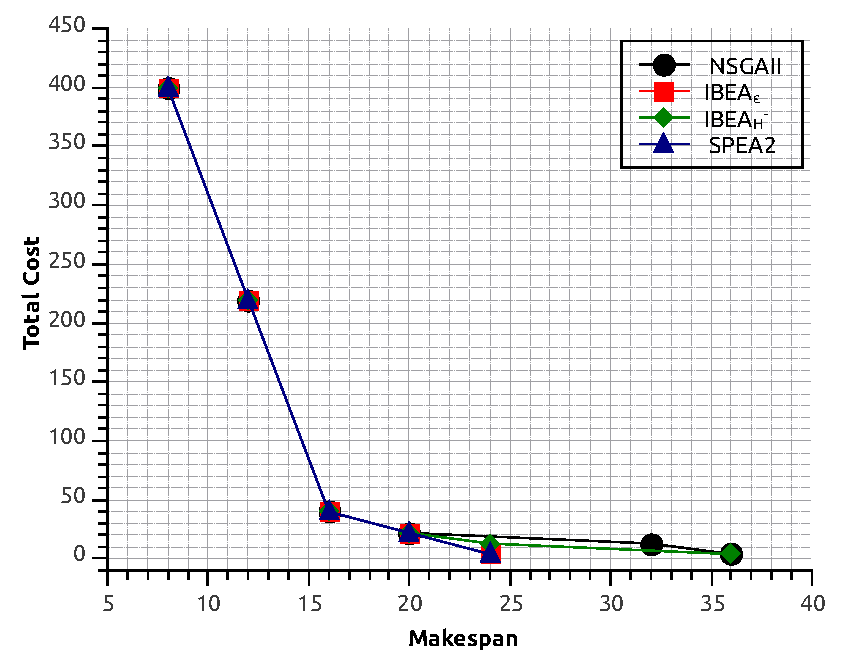
\includegraphics[width=0.41\textwidth]{./paretofrontZeno3Add.eps} %bb=0 0 388 304, scale=0.35
\label{fig1-a:zeno3AddParetofrontareto}}
\subfloat[Zeno6$_{cost}$]{ 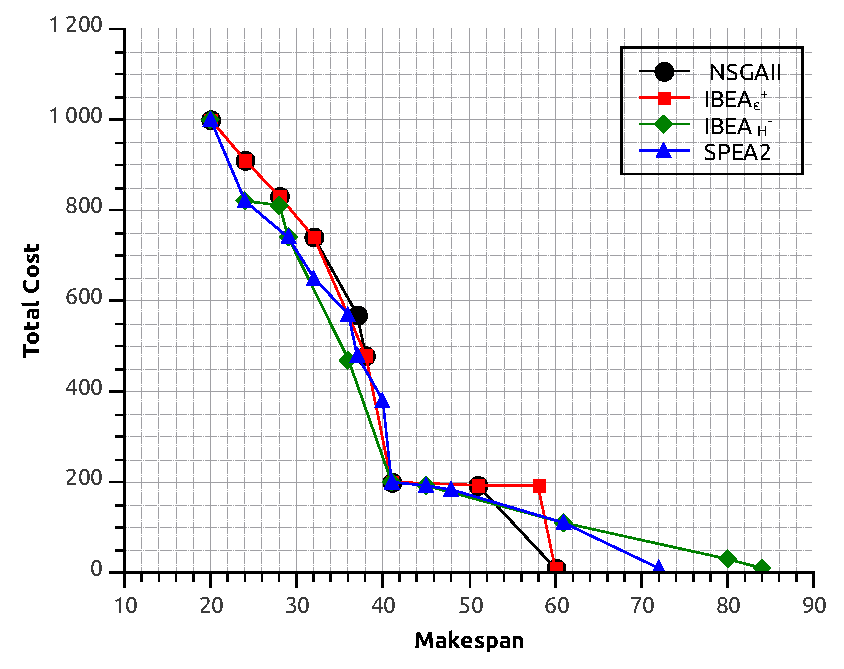
\includegraphics[width=0.41\textwidth]{./paretofrontZeno6Add.eps}%[bb=0 0 389 305, scale=0.35
\label{fig1-b:zeno6MaxParetofrontareto}}
\\
\subfloat[Zeno9$_{cost}$]{ \includegraphics[width=0.41\textwidth]{./paretofrontZeno9Add.eps}
 % paretofrontZeno9Add.eps: 0x0 pixel, 300dpi, 0.00x0.00 cm, bb=0 0 389 305
\label{fig1-c:zeno9MaxParetofrontareto}} 
 
 % nsgaZenoMax.eps: 0x0 pixel, 300dpi, 0.00x0.00 cm, bb=0 0 374 278 
 \caption{Pareto fronts of the zeno instances.}
 \label{fig:zenoParetofront}}
\end{figure*}
\begin{figure*}[h]
 \centering{
\subfloat[ Zeno3$_{cost}$]{ 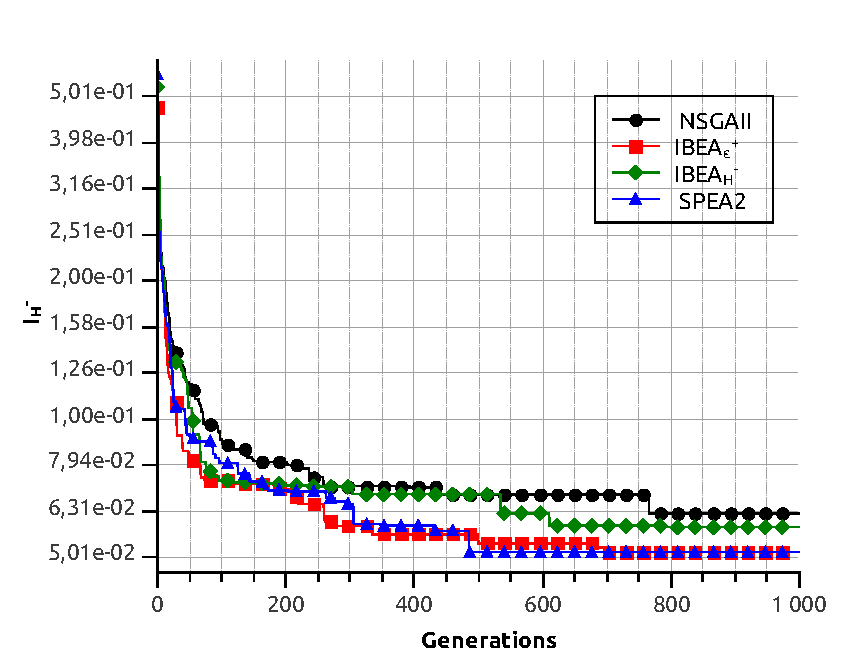
\includegraphics[bb=0 0 389 305,width=0.4\textwidth]{./hypervolumeZeno3Addmedian.eps}} %bb=0 0 389 305, scale=0.35
 % hypervolumeZeno3Addmedian.eps: 0x0 pixel, 300dpi, 0.00x0.00 cm, bb=0 0 389 305
 \subfloat[ Zeno3$_{risk}$]{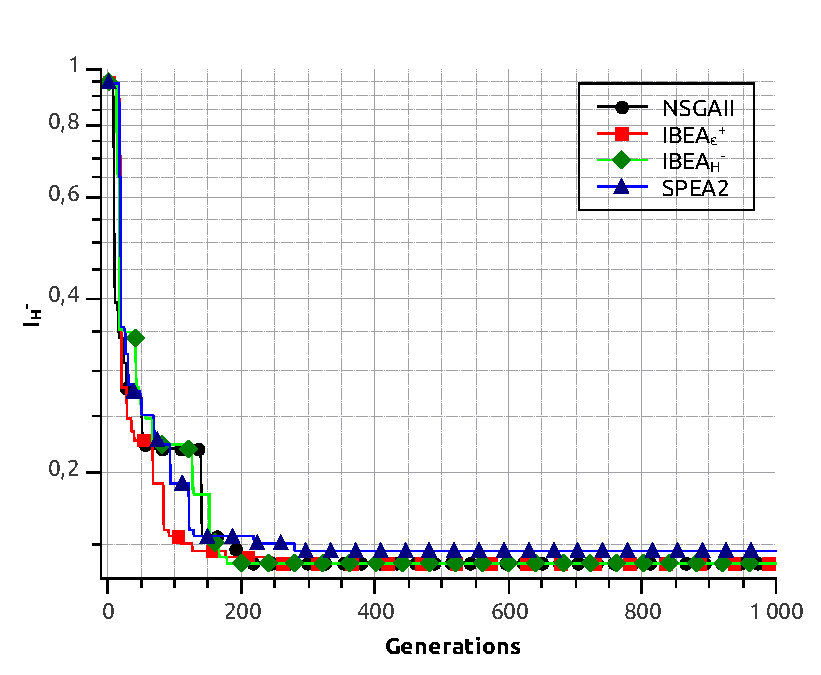
\includegraphics[bb=0 0 389 308,width=0.4\textwidth]{./hypervolumeZeno3Maxmedian.eps}}\\ %bb=0 0 378 308, scale=0.35
 % hypervolumeZeno3Maxmedian.eps: 0x0 pixel, 300dpi, 0.00x0.00 cm, bb=0 0 378 308
  \subfloat[ Zeno6$_{cost}$]{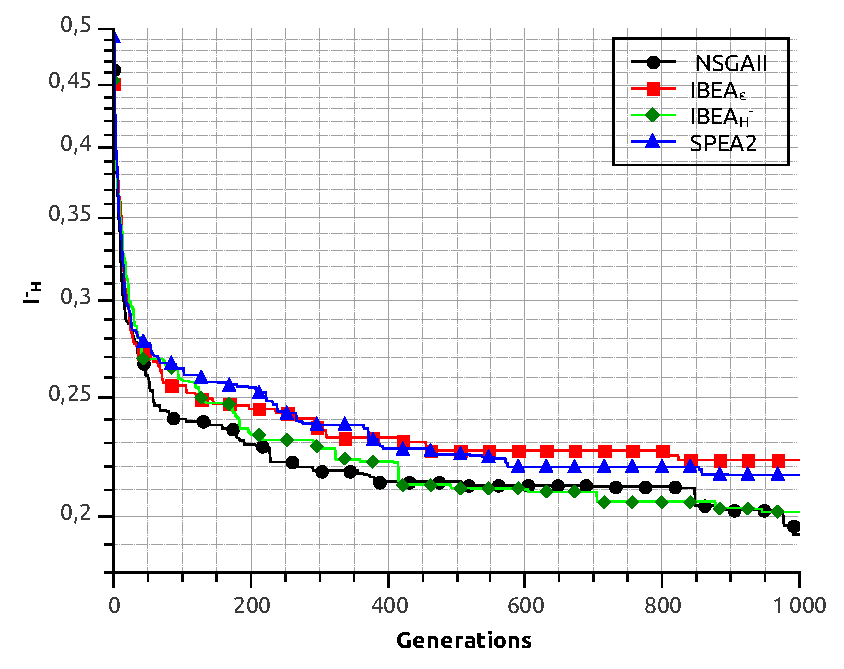
\includegraphics[bb=0 0 389 305,width=0.4\textwidth]{./hypervolumeZeno6Addmedian.eps}} %bb=0 0 389 305, scale=0.35
%  % hypervolumeZeno6Addmedian.eps: 0x0 pixel, 300dpi, 0.00x0.00 cm, bb=0 0 389 305
  \subfloat[ Zeno6$_{risk}$]{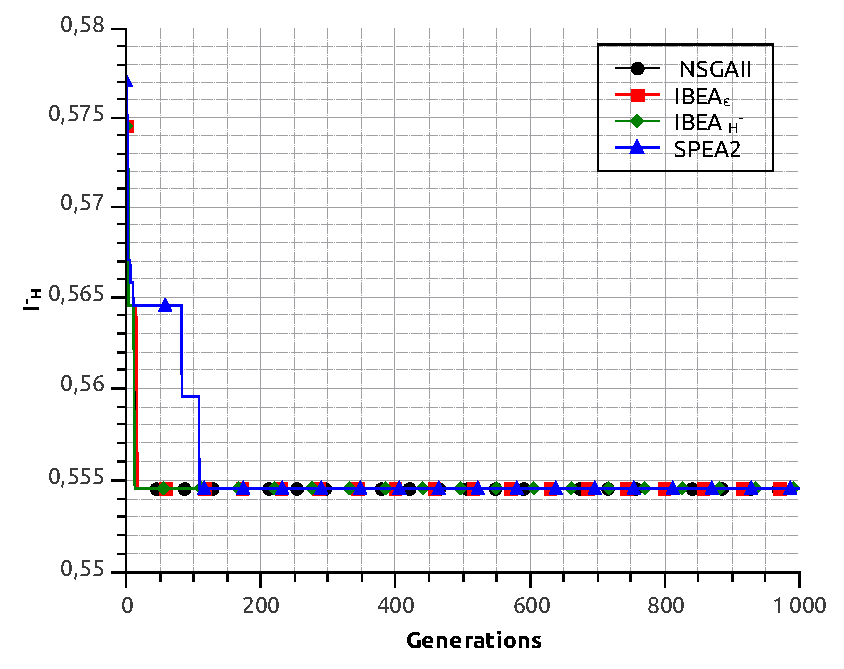
\includegraphics[bb=0 0 389 305,width=0.4\textwidth]{./hypervolumeZeno6Maxmedian.eps}} %bb=0 0 389 305, scale=0.35
%  % hypervolumeZeno6Maxmedian.eps: 0x0 pixel, 300dpi, 0.00x0.00 cm, bb=0 0 389 305
\\
   \subfloat[ Zeno9$_{cost}$]{\includegraphics[bb=0 0 334 269,width=0.4\textwidth]{./hypervolumeZeno9Addmedian.eps}}
 % hypervolumeZeno9Addmedian.eps: 0x0 pixel, 300dpi, 0.00x0.00 cm, bb=0 0 334 269
 \subfloat[ Zeno9$_{risk}$]{\includegraphics[bb=0 0 389 305,width=0.4\textwidth]{./hypervolumeZeno9Maxmedian.eps}}
  
\caption{Madian evolution of the quality of solutions on zeno instances  according to Hypervolume indicator $I_{H^-}$ over 30 runs.}

 \label{fig:zenoHypervolume}}
\end{figure*}



% 
% 
% \begin{figure*}[h]
%  \centering{
% \subfloat[ Zeno3$_{cost}$]{ 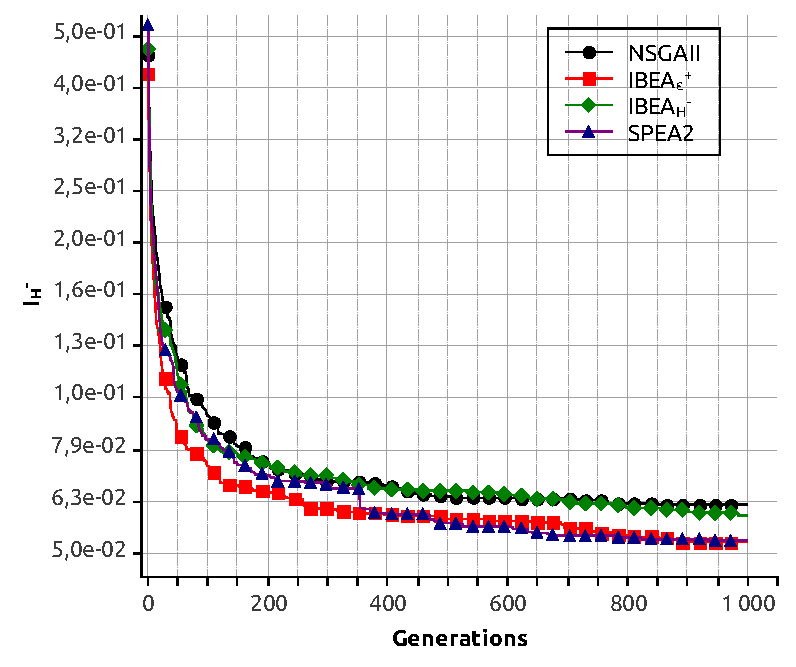
\includegraphics[bb=0 0 366 304, scale=0.45]{./hypervolumeZeno3AddAverage.eps}}
%  % hypervolumeZeno3Addmedian.eps: 0x0 pixel, 300dpi, 0.00x0.00 cm, bb=0 0 389 305
%  \subfloat[ Zeno3$_{risk}$]{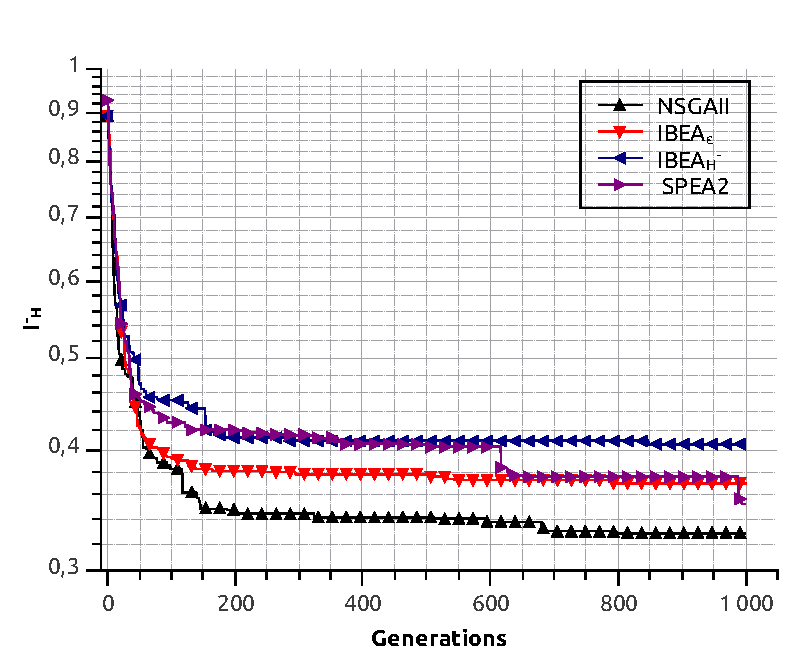
\includegraphics[bb=0 0 366 304, scale=0.45]{./hypervolumeZeno3MaxAverage.eps}}\\
%  % hypervolumeZeno3Maxmedian.eps: 0x0 pixel, 300dpi, 0.00x0.00 cm, bb=0 0 378 308
%   \subfloat[ Zeno6$_{cost}$]{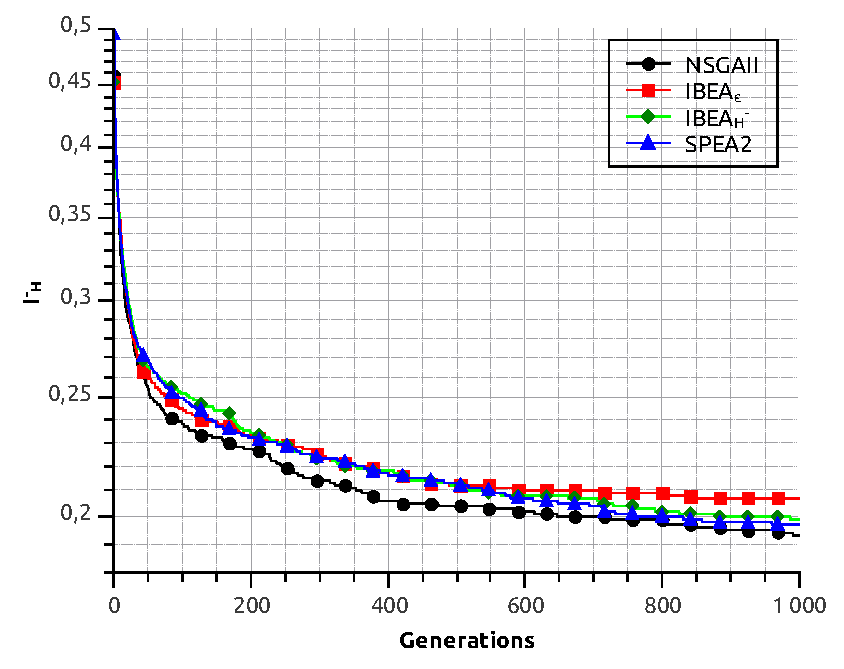
\includegraphics[bb=0 0 389 305, scale=0.45]{./hypervolumeZeno6AddAverage.eps}}
% %  % hypervolumeZeno6Addmedian.eps: 0x0 pixel, 300dpi, 0.00x0.00 cm, bb=0 0 389 305
%   \subfloat[ Zeno6$_{risk}$]{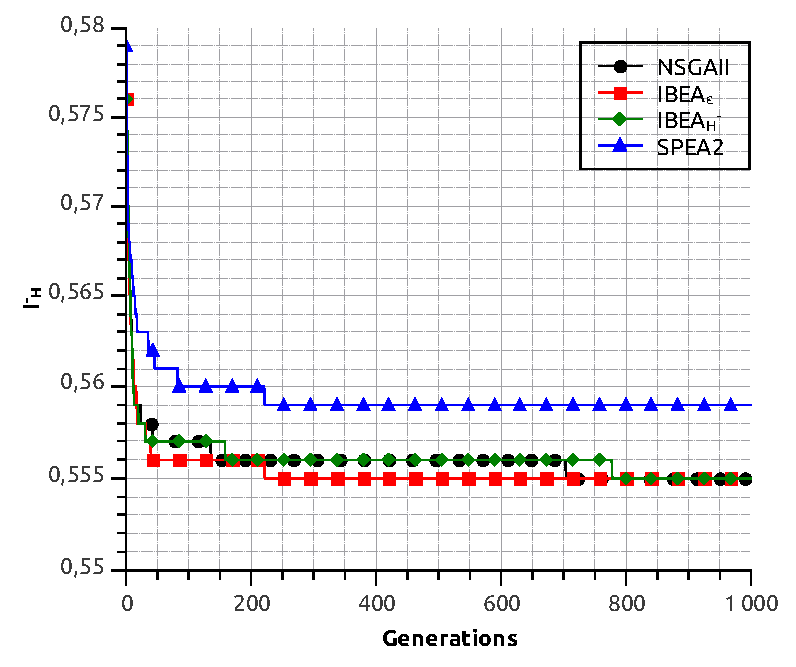
\includegraphics[bb=0 0 366 304, scale=0.45]{./hypervolumeZeno6MaxAverage.eps}}
% %  % hypervolumeZeno6Maxmedian.eps: 0x0 pixel, 300dpi, 0.00x0.00 cm, bb=0 0 389 305
% \caption{Average evolution of the quality of solutions on zeno instances  according to Hypervolume indicator $I_{H^-}$ over 30 runs.}
% 
%  \label{fig:zenoHypervolume}}
% \end{figure*}

\section{Conclusion \& Perspectives}
\label{sec:conclusion}
In this work we have proposed multi-objective algorithms based on Divide-and-Evolve strategy, which hybridizes
the behavior of an evolutionary  multi-objective algorithm with an embedded solver called YHASP. 
The approaches have been evaluated using a  new multi-objective zeno transportation benchmarks. 
As first objective, we have considered the makespan, where in the second objective
the total cost related to the travel or the risk have been considered.
The obtained results show that  depending on the size of the instance and the second treated objective (cost/risk),  the behavior of the algorithms changes.
A study of the behavior of the algorithms when applied to problems having more than two objectives  as well as the parallelizing of the multi-objective Divide-and-Evolve approaches are  a matter of future work.
\bibliographystyle{splncs}
\bibliography{ppsnb}


\end{document}
